%
% このファイルはヒューマンインタフェース研究報告集用クラスファイル
% hisken.cls(ver.1.0) を利用した「原稿執筆の手引き」です.
% Revised in Jun. 7, 2007 by Yutaka Ishii
%

\documentclass[a4paper,dvipdfmx]{hisken}
%\usepackage[dviout]{graphicx}
\usepackage{graphicx}
\usepackage{latexsym}
\usepackage{graphics}
\usepackage{epsfig} \let\epsfile=\epsfig
\usepackage{url}

%和文タイトル
\jtitle{ユーザの状態に共感的行動を示す協働エージェントによる孤独感への影響}

%著者日本名
\jauthor{
梅田 和希\thanks{関西大学 総合情報学部}   
}
%英文タイトル
\etitle{Effects on loneliness by virtual agent with empathic behavior to user's status}

%著者英文名
\eauthor{
Kazuki Umeda\thanks{Kansai University, Faculty of Informatics}
}
% 名前は,はじめの一文字だけ大文字にしてください.

\begin{document}

%maketitle は abstract と keyword の後に入れてください.

\begin{abstract}
本研究では, 孤独感を現代の先進国にある社会問題の一つとして取り上げ, それを軽減する手法として音で人間の存在感を模倣した仮想エージェントを提案する. そしてその存在に対して人間が感情移入をして, エージェントが人間の存在を代替し得るのか否かを検討する. その際, 孤独という概念は非常に主観的なものであり, また孤立などの密接に関係する近い概念と混同しやすい. よってまず初めに, 心理学の分野でそれらの定義や区別を試みた研究や調査を取り上げ, 本研究で取り扱う範囲を明確にする. 次に孤独が人間に及ぼす影響, そして主要な先進国に行われた孤独に関係する調査を取り上げる. そして最後に工学分野での関連研究と本研究でのエージェントについて述べる.
\end{abstract}

\begin{keyword}	
%%History, augmented reality, 3DCG, animation, learning support
孤独, 孤立, loneliness, 音, アンビエント, 存在感, キャラクター, 共感, 共感的行動, 協働, RNN, LSTM
\end{keyword}

\maketitle
	
\section{孤独の定義と扱う範囲}
孤独という概念は定義が曖昧なまま、漠然としたイメージで日常で述べられることが多い. しかしその実態は単一の心理状態ではなく, 孤立などの一見混同されやすい概念と複雑に重なりあっている. 解決する課題を明確にするため, まずここに心理学の分野で孤独とその周辺の概念がどのように定義されているのかを取り上げる.
\subsection{孤立と孤独}

CornwellとWaiteによる2009年の調査では, 客観的に社会からどの程度孤立しているかを示すSocial disconnectedness(社会的孤立)と, 主観的に交友, 交際関係や支援される対象に不足を感じているかを示すPerceived isolation(認知された孤立)にわけた{}\cite{tex1}. そしてそのそれぞれが精神的, 身体的にどの程度影響を与えるのかを調べた.(孤独については心理学的アプローチと, 社会学的アプローチがこれまでになされている. 前者は被験者の主観的な孤立の感覚に注目し, 後者が客観的に数量で表される指標で測ろうとするが, CornwellとWaitは, これまでその2つの軸を同時に扱って比較されていなかったことを課題とした.)

2014年にJohn T. CacioppoとStephanie Cacioppoによって行われた調査においても, 社会的孤立と健康状態の関係を調べる上で, 社会的孤立はObjective isolation(客観的孤立: 家族,や友人の数など, 数量化できる要素が要因)とSubjective isolation(主観的孤立)の2つの側面を持つとした{}\cite{tex2}. さらにSubjective isolationを前述のPerceived isolationという言葉で言い換え.それを孤独と同義として扱った.

\subsection{2種類の孤独}

また2018年にアメリカ人の18から70歳までの成人1800人を対象に行われた調査では, 孤独はSocial loneliness(社会的孤独)とEmotional loneliness(感情的孤独)の二つの軸に分けて考えられた{}\cite{tex3}.
Social loneliness(社会的孤独)とは, 自分の周囲にいる人の数に理想とのギャップを感じている状態である. 自分には親, 友達, また困った時に助けてくれる間柄の人がほとんどいないなどと感じていることが考えられる. それに対しEmotional loneliness(感情的孤独)とは, 関係を持つ人の数でではなくその質に満足していない状態を表す. 家庭を持っていたり, 多数の社会的繋がりを持っていても心理的な距離を感じたり, その繋がりが本人を消耗させる原因になっている場合も考えられる. 
この2つの軸から, 被験者の孤独感は以下の4つのサブクラスに分けられた. 
\begin{itemize}
\item Low loneliness: どちらの孤独感も主観的度合いが低い
\item Social loneliness: 社会的繋がりの量(数)に不満足である
\item Emotional loneliness:  社会的繋がりの質に不満足である
\item Social and emotional loneliness: 社会的繋がりの量(数), 質共に不満足である
\end{itemize}


このSocial loneliness(社会的孤独)は, CornwellとWaite(2009)やJohn T. CacioppoとStephanie Cacioppo(2014)らのいうPerceived isolation(本人が認知している孤立)と同様の概念を指すと思われる。

他にも多数の孤独や孤立を定義して調査した研究が存在するが, それらを集約すると以下の3つに分類されることが多いと考えた.
\begin{itemize}
\item Social disconnectedness / Objective isolation (以下, 社会的孤立状態とする.)
\item Perceived isolation / Subjective isolation (以下, 社会的孤立状態とする.)
\item loneliness (以下, 孤独感とする. 2と同義とされることもある.)
\begin{enumerate}
\item Social loneliness(以下, 社会的孤独とする. Perceived isolationおよびSubjective isolationと同義と考えられる.)
\item emotional loneliness(以下, 感情的孤独とする.)
\end{enumerate}
\end{itemize}


\section{孤独と孤立が人間に及ぼす影響}
現在調べ中. なぜそもそもそれらを問題視する必要があるのかという説明になるため, この部分は必要である. 

\section{先進諸国と日本の現状}
アメリカの, 国際的に医療と健康のサービスを展開する企業であるCignaが2018年の5月に発表した, 20,096人のアメリカ在住の18歳以上の人を対象に行った大規模な調査の結果{}\cite{tex4}がある, その一部に次の様なものがある. 
\begin{itemize}
\item 約半数の人が時々, または慢性的に孤独感を感じている(46%), また周囲から取り残されていると感じている(47%)
\item 約27%の人が自分のことを理解している人が全く, または殆どいないと感じている. 
\item 約43%の人が, 既にある人間関係に意義を感じていない, または周囲から孤立していると感じている. 
\item 他の人と共同生活をしている人(UCLA孤独スコア: 43.5) は, 一人で生活している人(UCLA孤独スコア: 46.4)に比べて孤独感が比較的軽い. しかし一人でなくても, 本人が片親や一人で身元引き受け人になっている場合, 子供と一緒に暮らしているにも関わらずより大きな孤独感(UCLA孤独スコア: 48.2)を感じている. 
\end{itemize}


この結果から, アメリカにおいて孤独や孤立の感覚は大多数の割合の国民に及ぶ社会問題と考えるのが妥当であると考える.

また, 同年10月にイギリスのBBCの主要なラジオ放送局の一つであるBBC Radio 4が行った. オンライン上での孤独に関する調査結果{}\cite{tex5} {}\cite{tex6}がある(国内のマンチェスター大学、ブルネル大学、エクセター大学の協力の元に行われた). 同調査では約55,000人の一般人からの回答が集まり, 孤独に関するこの類の調査としては世界最大規模となった. 
その結果, 16~24歳の年齢層が,他の年齢層に比べて最も孤独感を感じている人の割合が多いことが分かった(孤独感を時々/頻繁に感じると回答した割合が40%と, 最も多かった. 65~74歳は29%, 75歳以上は27%であった. ). 

日本では近年において, 国内で一般人を対象とした,孤独に関する信頼できる調査が少ないが, ”引きこもり”についての調査が存在する. 
内閣府は2009年と2015年に若年層(15~39歳)の, また2015年に中高年層(40~64歳)の引きこもりに該当する国内の人数を推定した調査{}\cite{tex7} {}\cite{tex8}を行っている. その結果, 若年層で54.1万人, また中高年層で61.3万人と推定された.
このことから, 我が国でもSocial isolation(社会的孤立)に相当する状態にある人が多数いると思われる.


\section{本研究で取り扱う範囲}
孤立感や孤独感を抱くシチュエーションは様々であり, それぞれで解決可能性や解決方法が異なる. しかしその多くは次の3つのタイプに分類できると考えた.

\begin{itemize}
\item 不協和: これはすでに持っている人間関係が, 本人の理想とする状態から離れている時に起こりやすい. 例えば, 学校で仲間集団からいじめを受けている状況や, 恋人や夫婦間などの親密な相手との関係が原因で精神的に疲弊している場合などである. この時, 周囲に助けを求めたり, 相談できる他者がいない場合にemotional lonelinessを抱くと考えられる.
\item 欠乏: これは自分が持っていない他者との関係を欲している状況で起こりやすい. 異性との親密な関係を欲していたり, 仕事の悩みを相談できる相手がいないといった状況などが考えられる.
\item 喪失: これはすでに持っている他者との関係が何らかの要因で失われた, または相対的にこれまでより極めて薄くなった時に起こりやすい. 長年連れ添ったパートナーとの死別や, 留学したことにより家族と長期間離れているような状況が要因として考えられる.
\end{itemize}

上の3つのシチュエーションのうち, 不協和に関しては既存の特定の個人, または集団間との人間関係の質の問題が要因となっており, そのエージェントによる解決策には, 人間関係を仲介する役割を担うものが考えられる. また喪失に関しては, エージェントによって既存の個人の存在の代替を担うことは現時点では考えにくいが, 特定の個人についてのポジティブな感情を思い起こさせる役割を持つエージェントなどが考えられる. 

しかし欠乏というシチュエーションの場合, 関係を欲する対象はしばしば不特定である場合がある. 物心がついた時から肉親がいないため, 授業参観日にクラスメイトが羨ましくなるといったものや, 親友の異性関係を見て, 同様の存在を欲するといったケースがそうである. これらのケースでは, 欲する人間関係の形態のモデルは存在するが具体的な個人または集団は存在しない. よってここに擬人化された仮想エージェントが人間の存在を代替する可能性があると考えた. よって本研究では欠乏に焦点を絞って擬人化エージェントの属性や人格的特徴を作っていきたい.



\section{提案システム}
\subsection{システム概要}
本研究では, エージェントに高いアンビエント性を持たせたい. このシステムの実装の仕方の可能性を考えると, 通常スマートフォンアプリ内のキャラクターが考えられる. この場合ユーザがアプリを起動して, こちらから画面に映るキャラクターに働きかけ, それに対しキャラクターが応答/質問したりといった流れが思いつく. しかしここでの 始めのユーザからの能動的な行動により, そのキャラクターに対してメディアの等式が成り立たなくなり, 十分に感情移入できないのではないかと考えた. そのため, ユーザがそのキャラクターの存在をよりリアルなものに感じられる様に, システムをより実空間に溶け込んだものにし, さらにユーザに対してキャラクター側からも能動的に働きかけられる様にしたい.

関連研究としては2006年の板垣らによる音でエージェントの存在感を創出してユーザとインタラクションをさせた研究{}\cite{tex9}が挙げられる. ここでもユビキタス社会の到来を想定して, 小川らの提案するITACOシステムを発展させる目的でアンビエント性の高い音でエージェントの存在感が作られた. しかしここではユビキタス環境の中で, システムが常にユーザのアテンション(注意)を引きつけることを重要視されている. しかし現実の日常ではユーザが起きている間, 常にエージェントとやりとりをしている状態は考えにくい. メディアの等式が働き, ユーザがエージェントに対して感情移入ができるのであれば, 同時に, そのエージェントに対して自らのプライバシーの必要性なども感じるのではないだろうか. また, ユーザが何らかの作業に集中しているときにエージェントが存在感を強くしすぎることも好ましくない. よってここではユーザの状態に応じてエージェントの音の大きさなどのパラメータを動的に変動させて存在感を調整でき, 上手く環境に溶け込むことがでいるエージェントの政策を目指す.

欠乏し得る人間関係は個人によって様々であり, それぞれについてエージェントの性格的属性や内部の心理状態, 身体的特徴などを変える必要がある. また, 欲する関係の親密度によって, 要求されるそれらの作りこみの度合いも変化する. 

本研究では, 浅い関係である"協働仲間", そして比較的濃い関係である"友達"の2つの人間関係の形態に着目してエージェントを作っていく. 前者は会社のオフィスや大学での作業場などで, 壁の向こうでユーザと同じような作業をしている人間の存在感を音や光を使って模倣する. このエージェントは, 一人で室内で作業をしている人が孤独感を抱いているケースにおいてその感覚を軽減する目的で現在開発中である. 後者は作業をしている人の背後の空間を活用して, 親近感のある存在感を音で演出する. こちらは一人で暮らしているお年寄りや, 何らかの要因で一人での生活を余儀なくされている状況の人が孤立感, 孤独感を抱いている場合にてそれらを軽減する目的で開発している.

\subsection{システム構成}
どちらのシステムも, ユーザとインタラクションをするために何らかのインプットによりユーザの状態を把握する必要がある. 今回はユーザからのインプット取得のため, face-api.jsを使っている. 

face-api.jsはVincent Muhlerによって2018年に公開された, JavaScpitのAPIである. 機械学習のフレームワークであるtensorflow.js coreによって実装されており, webcamの映像から顔の位置の検出のほか, 輪郭の検出や, 性別や登録された個人の判断, neutral(無表情), happy(幸福), angry(怒り), sad(悲しみ), disgust(嫌悪), surprised(驚き), fearful(恐怖)の7つの感情値の推定など多様な機能を容易に導入することができる(図1参照). 明記されてはいないが, この7つの変数名から, おそらくアメリカの心理学者であるPaul EkmanとWallace V. Friesenの提唱されて広まった6感情のモデルが基になっていると思われる.

現在はシステムへのインプットとして上にあげたface-api.jsの機能のうち, 感情値の検出と顔の輪郭の検出の2つを使っている. またその2つの検出は0.2秒ごとに設定している.

\begin{figure}
  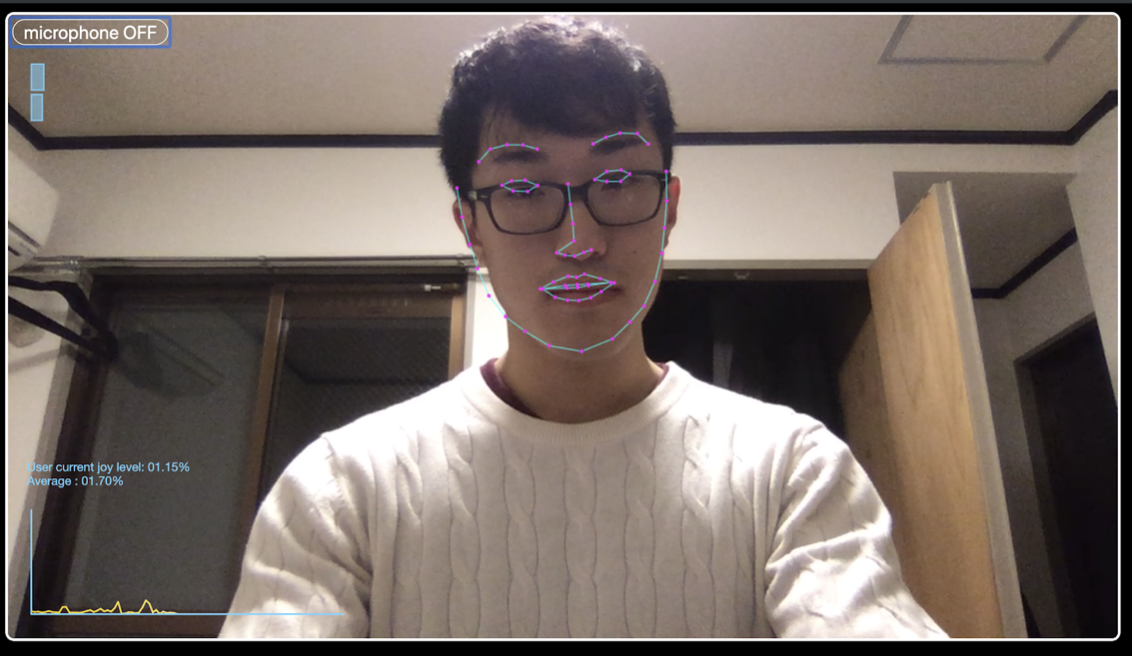
\includegraphics[width=\linewidth]{detection00.png}
  \caption{顔の検出と感情値の推定. 下で述べる協働仲間エージェントの開発中のUIである.}
  \label{fig:detection}
\end{figure}

また, 図1のように取得した感情値の数値やUIをブラウザ上で表示したり, エージェントの行動を実装するのにはp5.jsを使った. p5.jsは元々はcreative coding(実用性, 機能性などではなく, 視覚的に面白い表現を追求するためのプログラミング)のために作られたJavaScpitのフレームワークである. デフォルトで毎秒60フレームの処理が繰り返される関数が用意されており, それを利用することでエージェントの行動を時間志向でプログラミングすることが容易になると考えた(例: 単位時間でのユーザの顔の動きの平均が100pixelを超えると, その時点から30フレーム後(約0.5秒後)にエージェントの足音が聞こえる). 

\begin{enumerate}
\item 協働仲間エージェント
図2は現在開発中の協働仲間エージェントのシステムのハードウェアである. 作業をしているユーザの正面に外付けのwebcamを置てユーザの顔の映像を取得してface-api.jsで推定する.このシステムの具体的な処理の流れは, 

\begin{enumerate}
\item ユーザの感情値, 及び顔の動きを検知.
\item 1のインプットからユーザの内部状態を推定
\item エージェントの行動に関わる関数の発動, パラメータの大小の判定
\item 関数の発動
\item 壁の向こうからエージェントの音がユーザに聞こえる.
\end{enumerate}
というシンプルなものになっている. 

\begin{figure}
  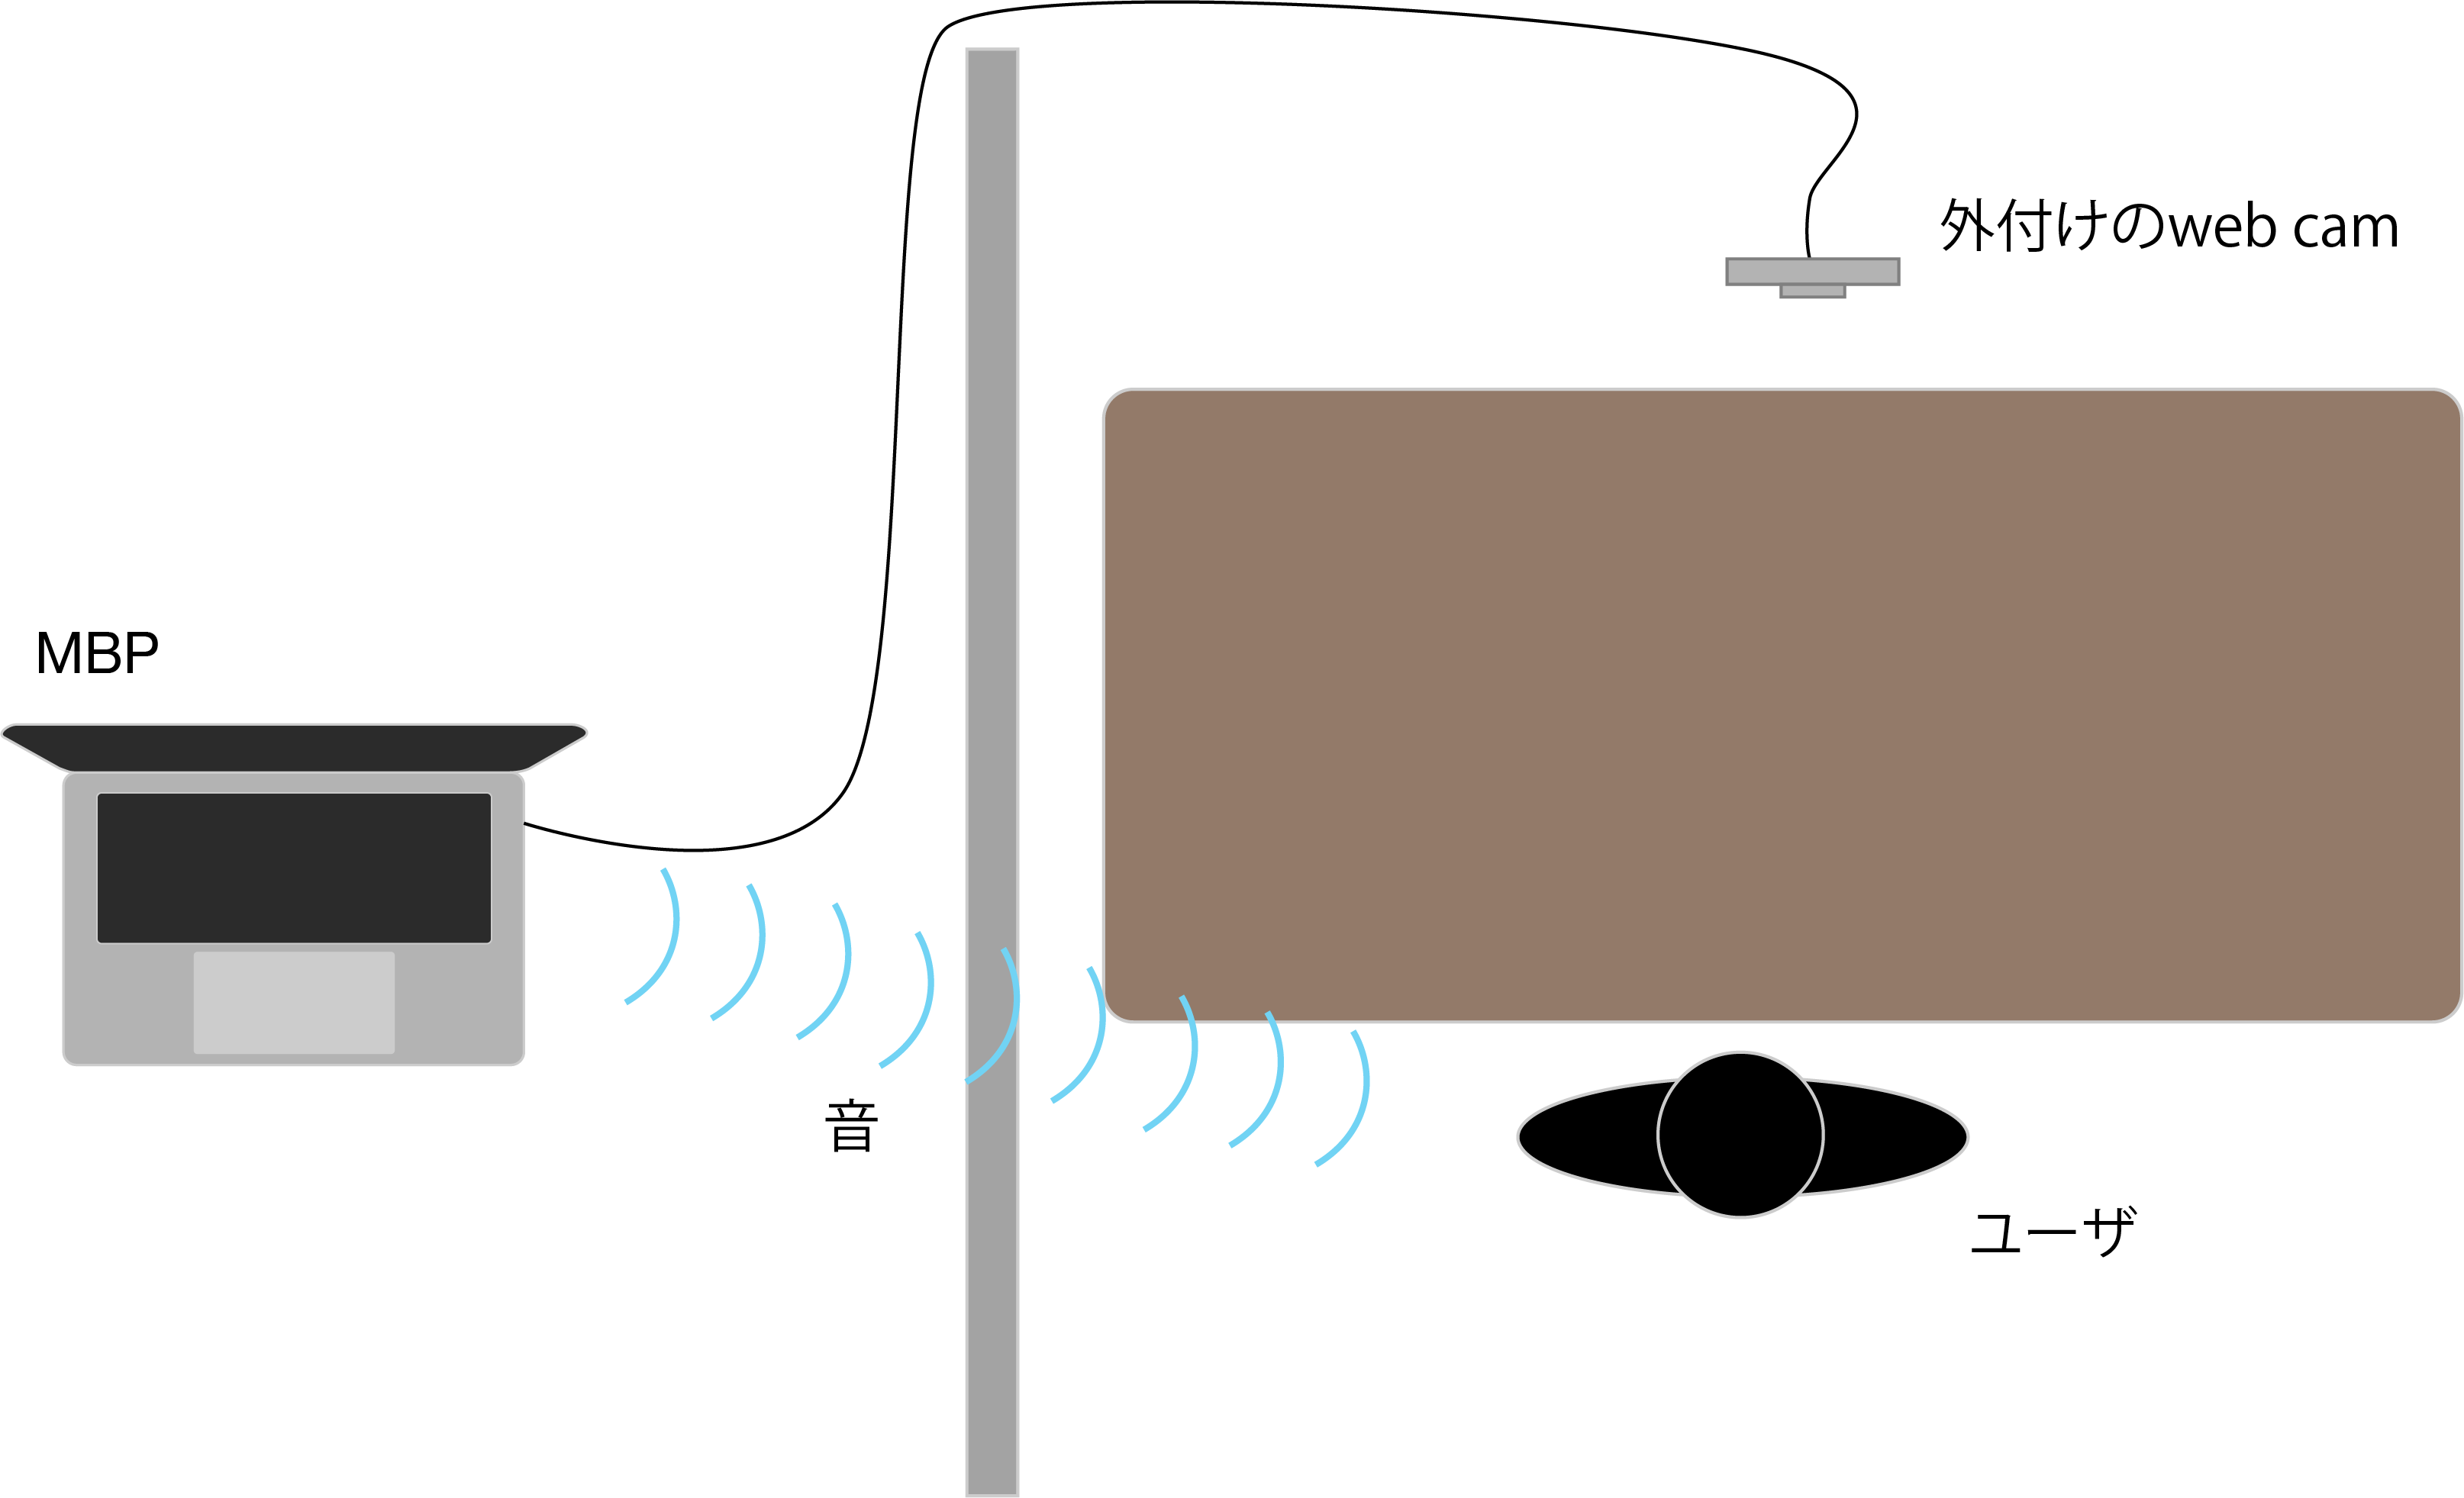
\includegraphics[width=65mm]{StrangerAgent_hardware.png}
  \caption{協働仲間エージェントのハードウェア}
  \label{fig:detection}
\end{figure}

aについて, ユーザの感情値についてはface-api.jsで7つのそれが取得できると述べた. しかし筆者がこのface-api.js感情値の推定を試したところ, neutral(無表情), happy(幸福), surprised(驚き)については非常に検出する感度が高いが, それ以外については顕著に低いことがわかった. 日常では考えにくい, あからさまな表情をしないと中々その感情の数値が上がらないという状態である. 

よってここではシステムの簡略化のためもあり, 7つのうちのhappy(幸福)のみを使うことにした. 顔の動きについて, face-apiでは図1のように, 顔の輪郭を検出して顔の64箇所の位置が推定される(ピンク色のドットで示されている部分). その64箇所のうち, 鼻の部分の一つのドットのxy座標を配列に格納して過去5フレームの平均を出してそれをinputとした. ここで平均値を取っているのは, inputの数値の変動の仕方を緩やかにするためである.

bおよびcについて, 孤独感を抱いている時の表情の変化や体の動き等については筆者の調べが進んでいないのだが, とりあえずここではhappyの数値と顔の位置が動いた距離が一定の値よりも小さければ, ポジティブな感情が薄く, 活動的ではないとして, その時に孤独感に浸っている可能性が高いとした. 

エージェントの関数について, 現在はエージェントがコンピュータのキーボードを叩く物理的な音, そしてスマートフォンでタイプする電子音の2つを実装している.  ユーザのhappyの数値と顔の動きが一定の閾値より小さいときにそれらの関数が発動し, ランダムにキーボードかスマートフォンのタイプ音が聞こえるようになっている. また, その関数の発動条件が満たされているとき, インプットの数値が小さいほどエージェントの音を大きくなるようにした. これにより, ユーザの状態に応じてエージェントの存在感の強さを調整できるようになった.

\item 友達エージェント

図3は現在開発中の友達エージェントのシステムのハードウェア, 図4はそのソフトウェアである. 

\begin{figure}
  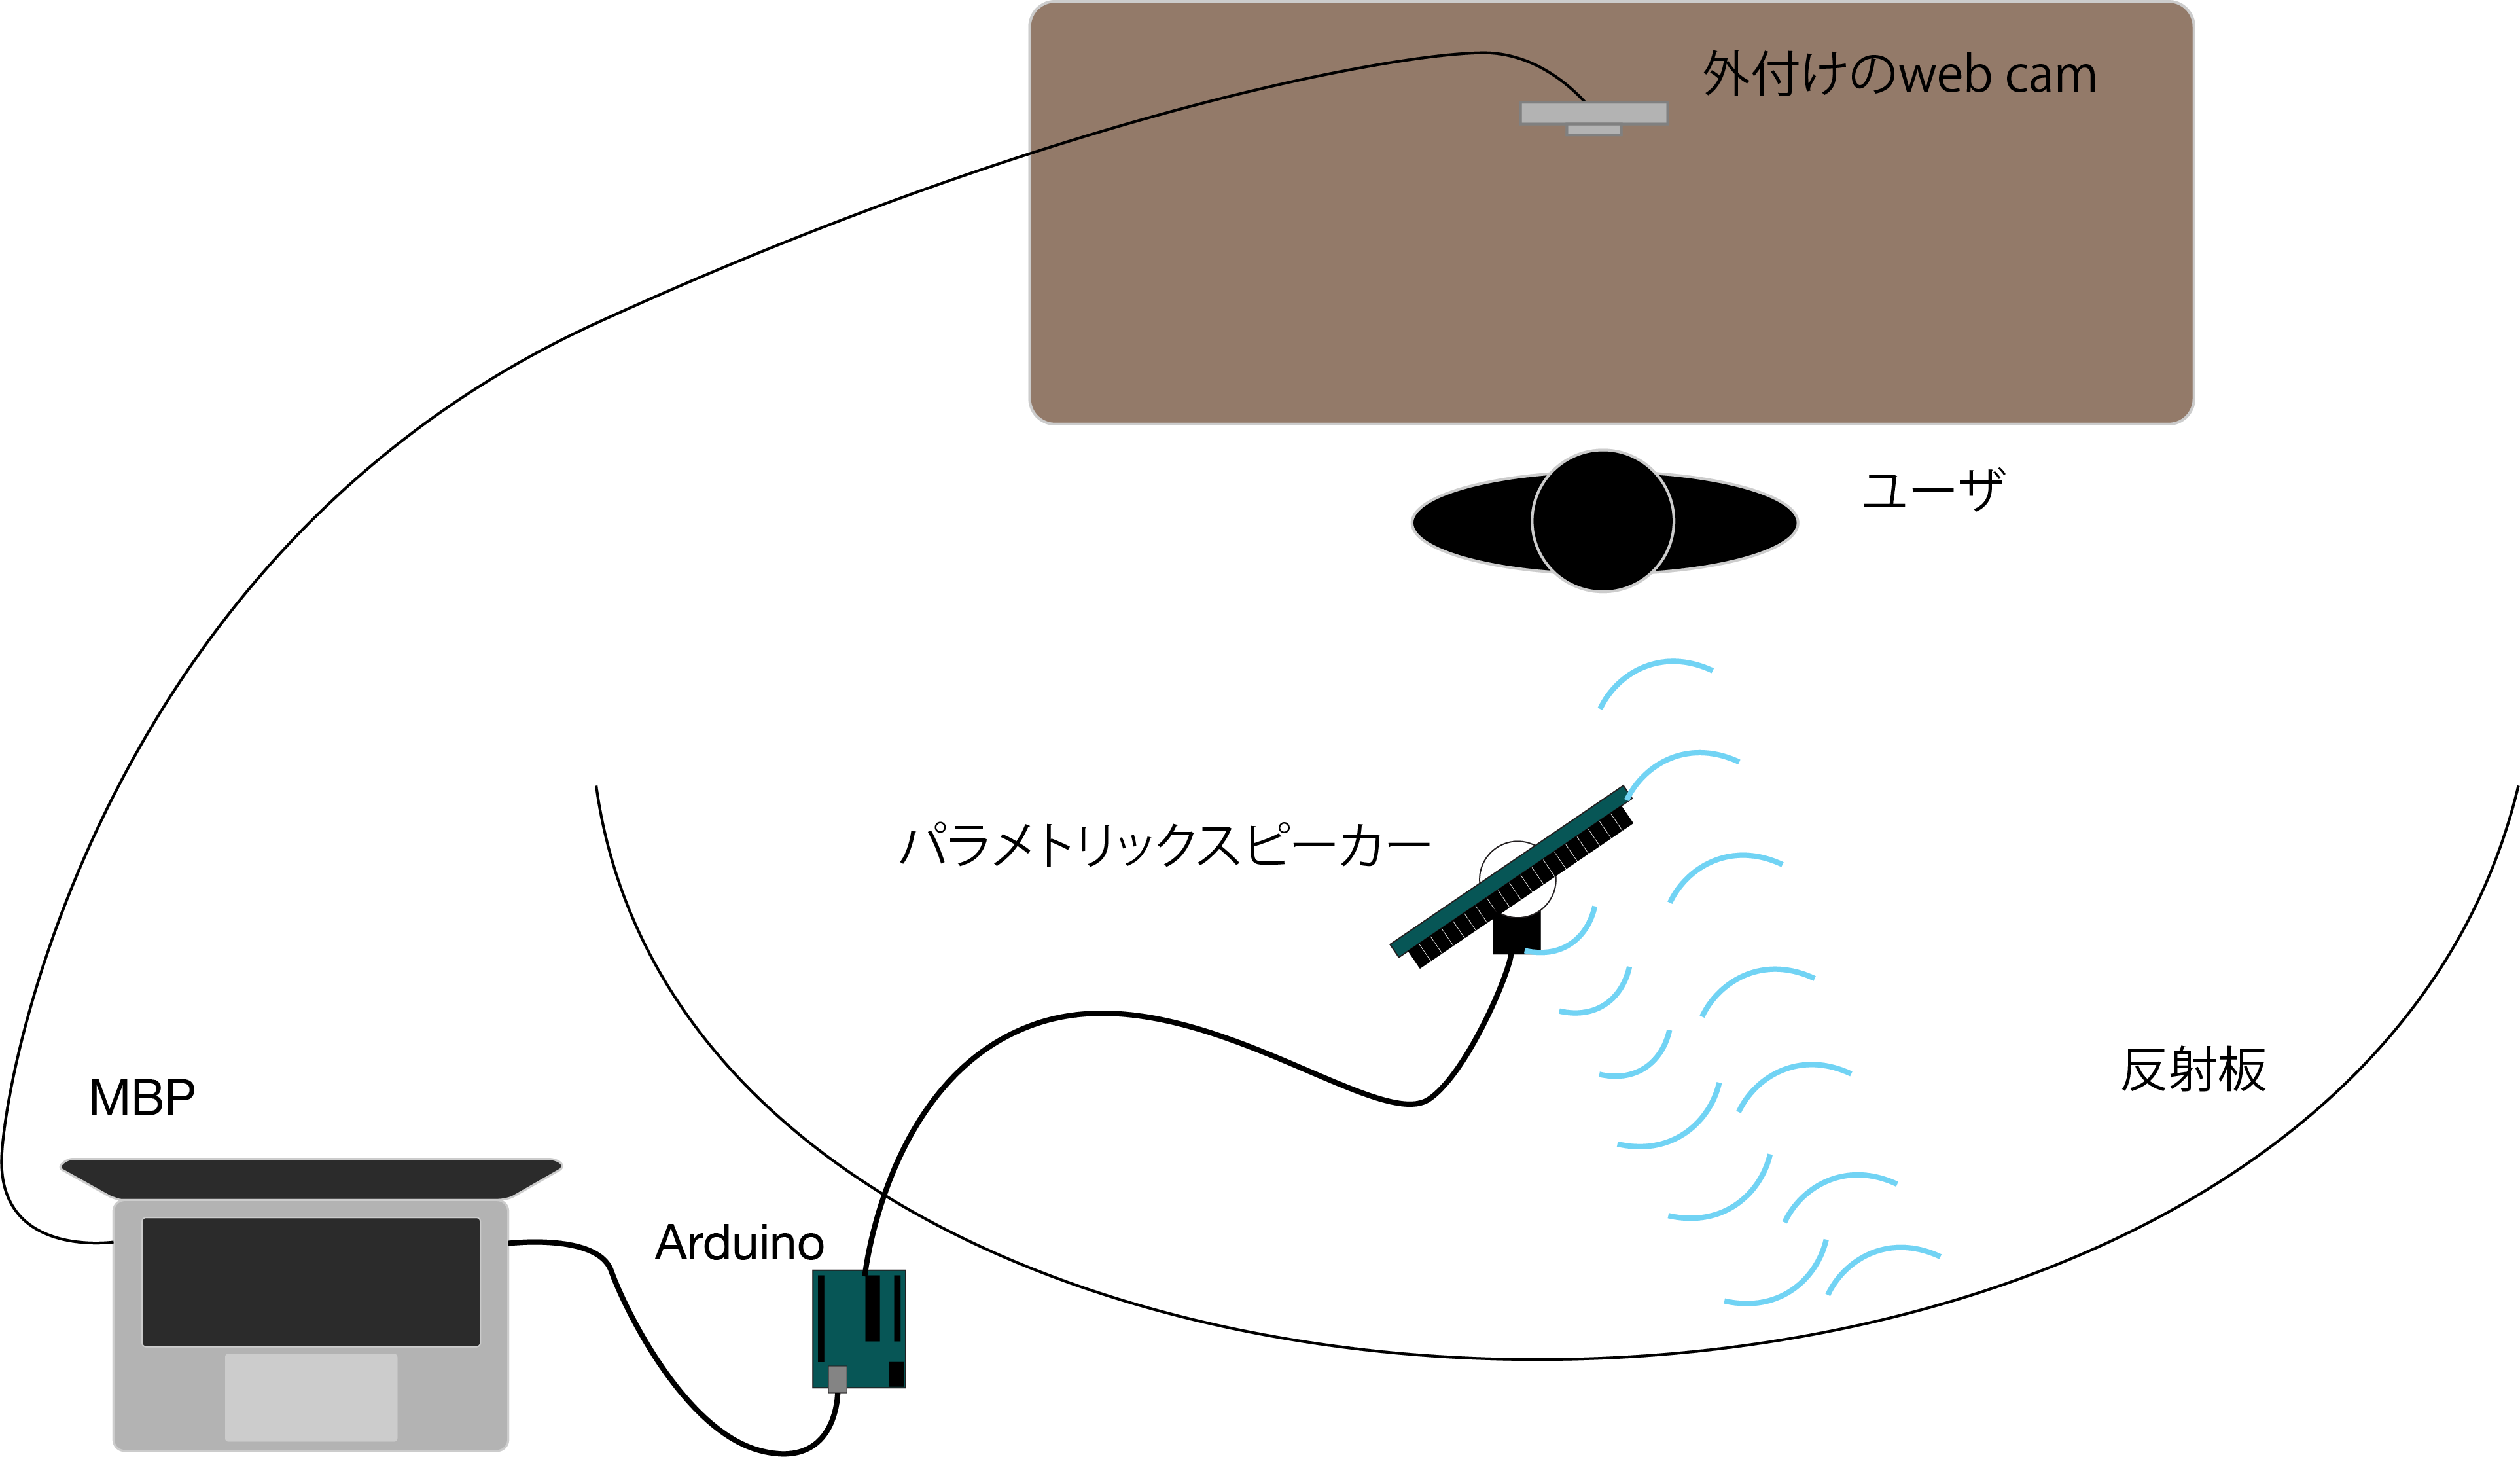
\includegraphics[width=\linewidth]{IntimateAgent_hardware.png}
  \caption{友達エージェントのハードウェア}
  \label{fig:detection}
\end{figure}

協働仲間エージェントと違い, 友達エージェントは存在感を感じる距離をより近くしたかったため, ユーザの背後の空間を利用することにした. まず図3のように, ユーザの背後から少し離れた位置に半円状の大きなスクリーンを設置する. そしてユーザとスクリーンの間に, 音を通常のスピーカよりも直線的に飛ばすことのできるパラメトリックスピーカーを設置する. パラメトリックスピーカーはArduinoを通してコンピュータとつながっており, コンピュータ内のコードから生成されたタイミングで音がそのスピーカーから流れるようになっている. 

\begin{figure}
  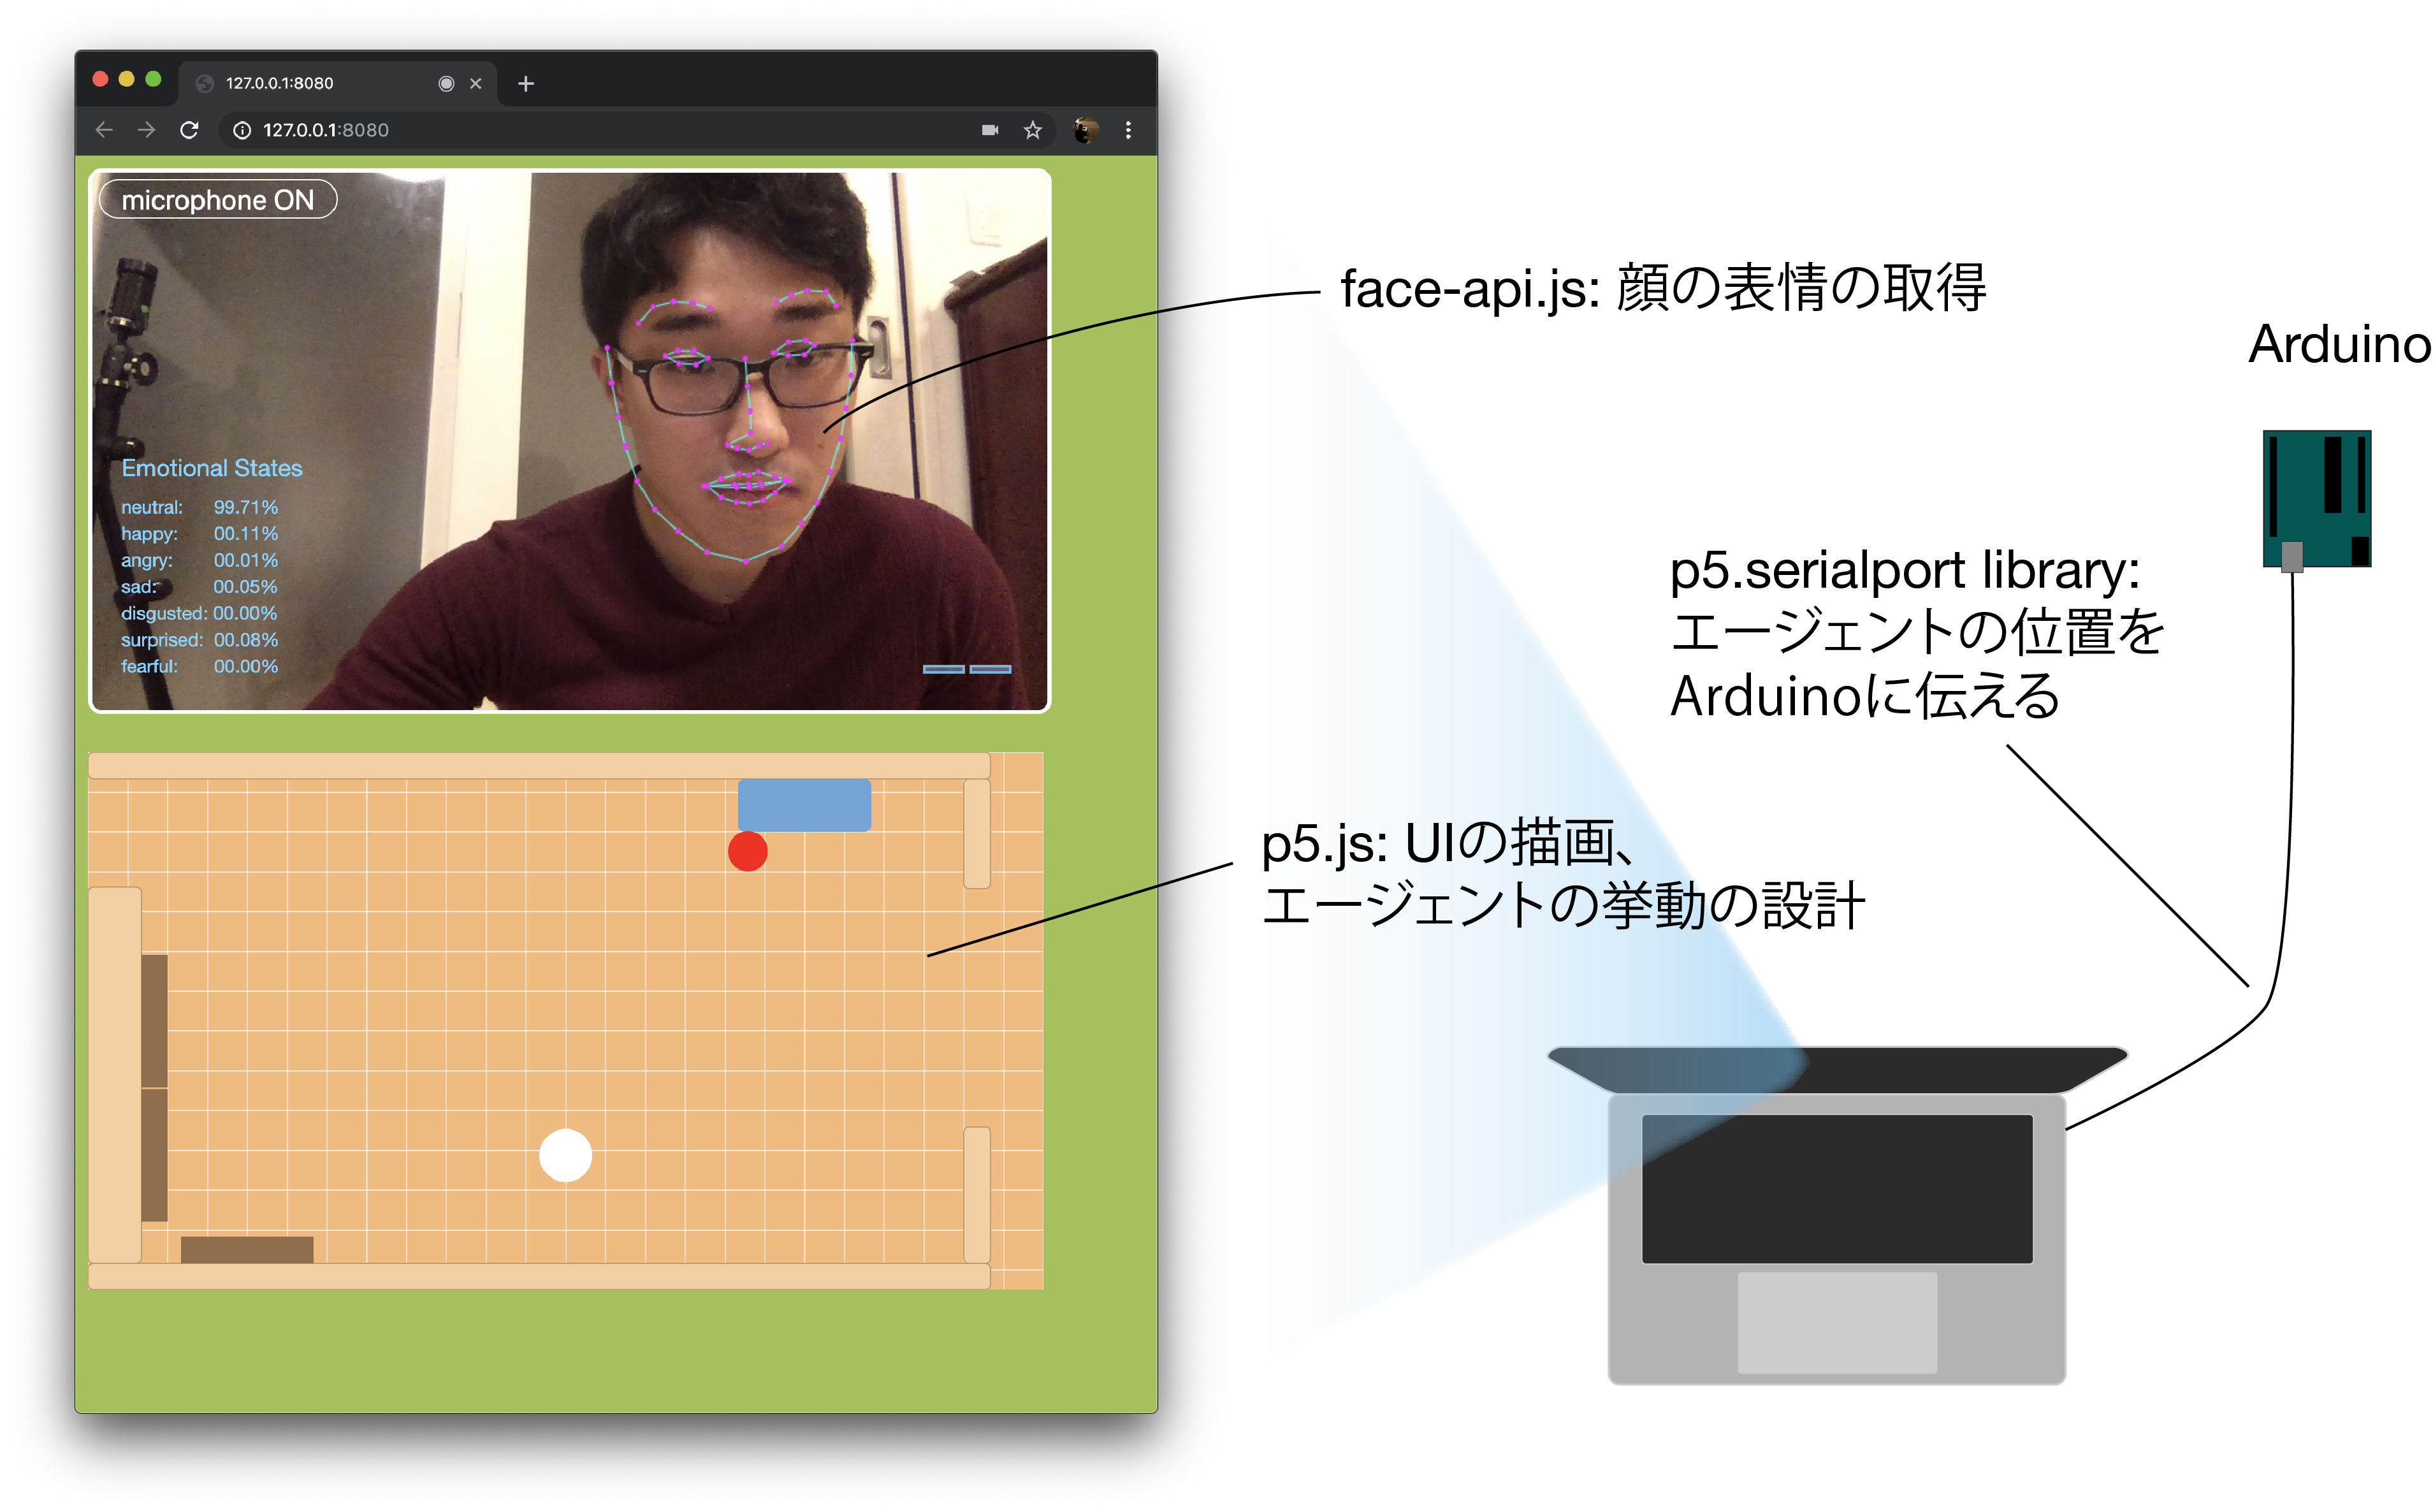
\includegraphics[width=\linewidth]{IntimaterAgent_software.png}
  \caption{友達エージェントのソフトウェア}
  \label{fig:detection}
\end{figure}

さらにパラメトリックスピーカーの下には, 回転する角度をコードによって自由に調節できるサーボモータを設置している. 図4の左の薄い黄色の部分のように, コード上ではユーザの周辺を上から仮想空間を作っており, その中でエージェントは自由に動く(図4では白い点がユーザ. 赤い点がエージェントの現在位置を表示したものである). 仮想空間内での, エージェントとユーザの相対的な位置関係に応じてJavaScriptのプログラムからArduinoを操作してサーボモータを回転させた. そのため, サーボモータが回転しながらエージェントの足音を出力すれば, ユーザからはまるで人が自分の後ろにいて移動しているかのような感覚を覚えることができる. 図5は筆者が制作した, パラメトリックスピーカーとサーボモータを一体化させた装置である. 

\begin{figure}
  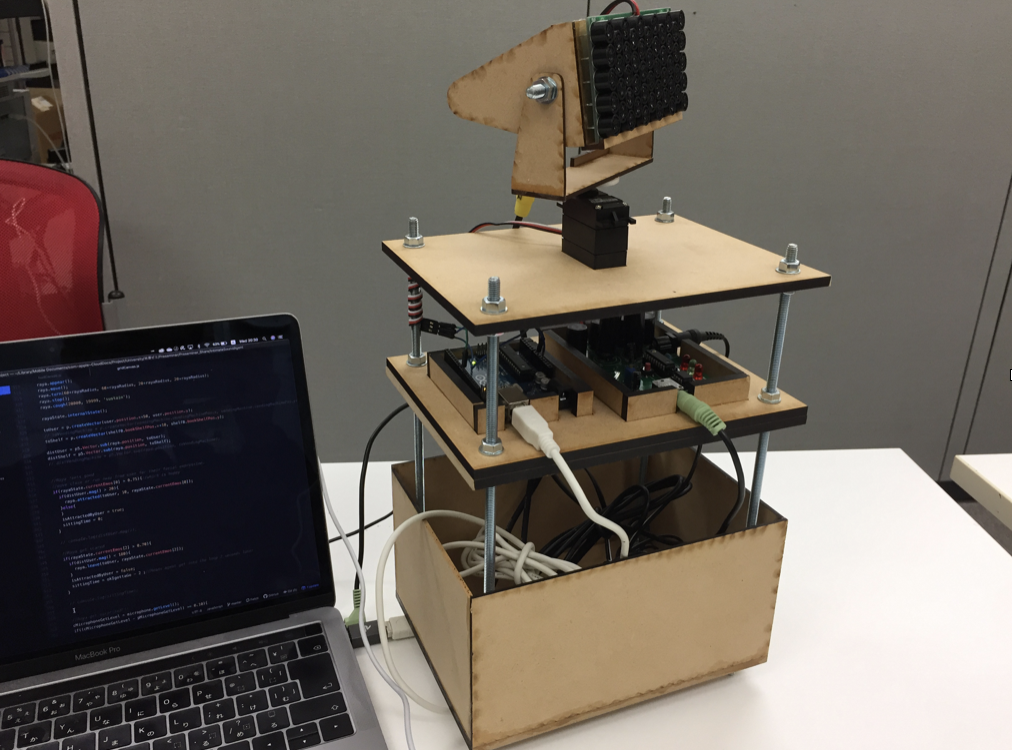
\includegraphics[width=\linewidth]{Speaker.png}
  \caption{友達エージェントの音を出力させる装置}
  \label{fig:Speaker}
\end{figure}


エージェントの内部モデルは現在未完成であるが, 想定するシステムの処理の流れは以下の通りである.

\begin{enumerate}
\item ユーザの感情値, 及び顔の動きを検知.
\item 1のインプットから人間の感情モデルにマッピングをしてユーザの内部状態を推定.
\item ユーザの内部状態からエージェントの内部状態を生成
\item 内部状態に応じて関数の発動, パラメータの大小の判定
\item 関数の発動
\item 上の処理と同時に, エージェントとユーザの相対的な位置関係によってサーボモータを回転させる.
\item 反射板によって音が反射してユーザにエージェントの存在感が伝わる.
\end{enumerate}


aについて, これは前述した協働仲間エージェントとほぼ同様である. 場合によって, p5.jsのsoundライブラリを用いてユーザの立てる環境音や, Kinect V2を用いてユーザの姿勢などもインプットとして扱う可能性もある.

bについて, ユーザのインプットの数値をRussellの感情円環モデルにマッピングすることも検討している. Russellの感情円環モデルは, 1980年にJames A. Russellが提唱した, 人間の喜びや悲しみ, 怒りなどの様々な感情を2次元座標上に分布させたモデルである{}\cite{tex10}(図5. この図は{}\cite{tex10}より引用した). 座標の横軸が快感 - 不快, 縦軸が心理的な覚醒の度合いを表す. しかしface-api.jsの7つの感情の変数はRusseellの感情円環モデル上では均等な分布ではなく, このシステムのインプットにある顔の動きなども含めてどのようにマッピングをするのかについては今後考える必要がある.

\begin{figure}
  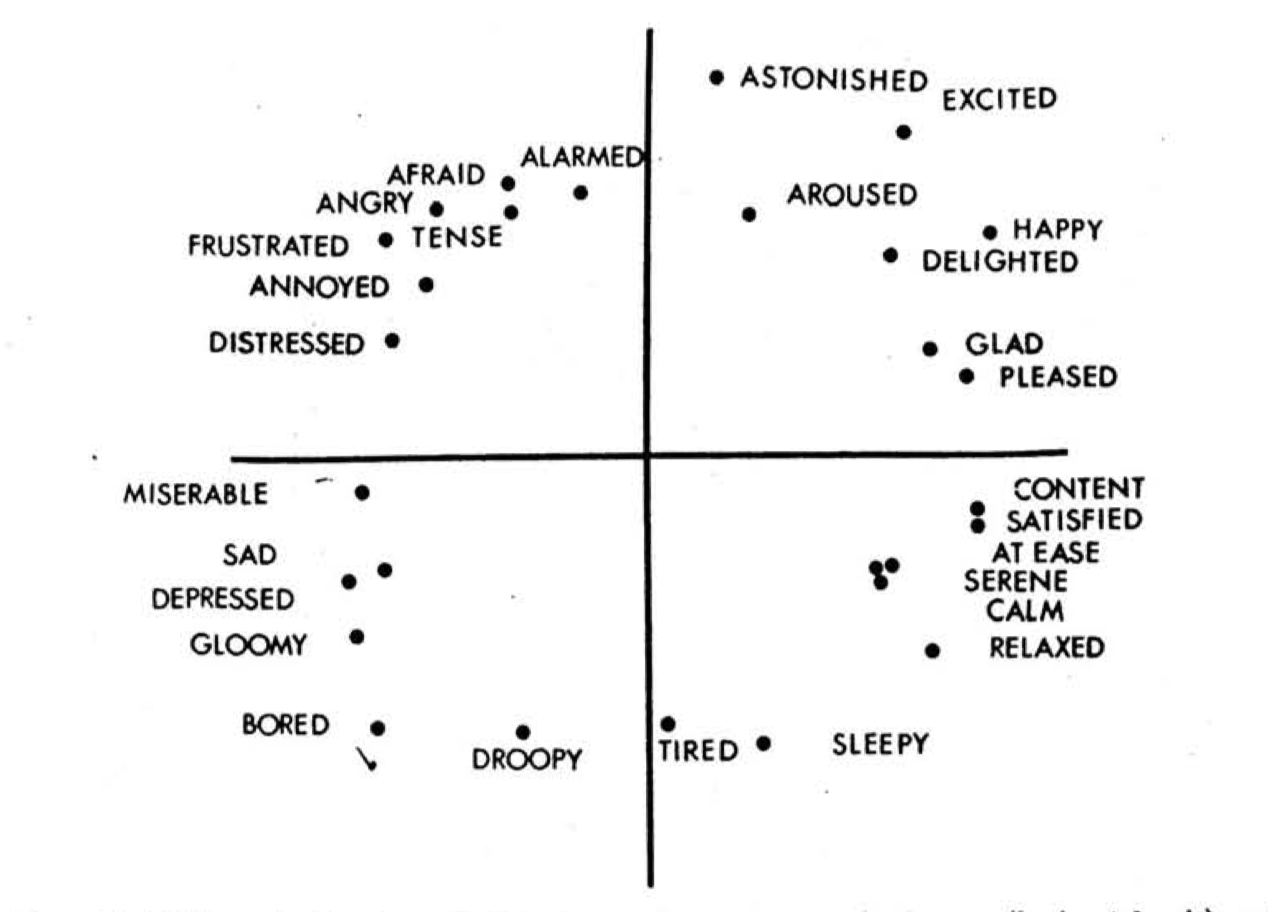
\includegraphics[width=\linewidth]{CircumplexModel.png}
  \caption{Russellの感情円環モデル}
  \label{fig:CircumplexMode}
\end{figure}


cについて, 友達エージェントは協働仲間エージェントよりも親密な関係をユーザとの間に構築する. 既に述べた協働仲間エージェントの場合, 存在感は提示するが, ユーザとの直接的なやりとりはなく, あくまで近くにいる他人であったので内部状態はそこまで要求されない. しかし比較的親密な友達と呼べる関係を作るには, 外界環境からのインプットによってエージェント自体の内部状態を生成するモデルが必要であると考えた. 

エージェントの内部モデルについて, 現在はハードコードで簡単なものをすでに作っている. まず, ユーザの過去5回分の7つの感情値の平均値をとる. 平均値をとる理由は協働仲間エージェントの部分で述べたように, 値の変動を緩やかにするためである(その方がエージェントの挙動の変化がスムーズに見える). 次に,  7つの平均値にそれぞれ, 0以上1.5程度の数字を乗算する. 例えばhappy(幸福)に1.25を, 怒りに0.75を乗算するならば, 結果としてエージェントはユーザの行動から幸せを感じやすく, 怒りを抱きにくいといった性格特性となる. 

次に, 性格特性の値を乗算された値に過去の残留感情を加算する. ここでの過去の残留感情とは過去900回分(約180秒分)のエージェントの7つの数字(ユーザの値 × 性格特性 + 残留感情)をある減衰グラフで畳み込みをさせたものの平均値である. 3次, 4次関数など高次元の数式を用いて波打った減衰グラフを作ることにより, 一度は収まった感情が後でぶり返すなどの人間的な感情の経過が表現できると考えた. 現在はこの数式は7つの感情値にそれぞれ別のものを用意して実装している. 発展として, この数式自体をユーザとのインタラクションの中で変動させるというアイディアもある. 

また, LSTMを用いて, ユーザの感情値の時系列データからエージェントの感情値を生成するというアイディアもある. そのため筆者は現在, O'REILLYの発行する著書"ゼロから作る Deep Learning"とその続編にてニューラルネットワークを学習中である.

\end{enumerate}


\section{終わりに}
孤独感を軽減させることを目的としてこの研究を続けているが, 筆者自身が孤独や孤立, および共感的行動などに関する知識が少ないと感じている. そのため, 今後John CacioppoやDilip Jesteといったそれらに関係する研究者の著書等を読み, 学習する予定である. また, ヒューマンエージェントインタラクションの分野についても学習を進める.

\begin{thebibliography}{99}
\bibitem{tex1}
	Erin York Cornwell, Linda J. Waite:
	Social Disconnectedness, Perceived Isolation, and Health among Older Adults.
	
\bibitem{tex2}
	John T. Cacioppo, Stephanie Cacioppo:
	Social Relationships and Health: The Toxic Effects of Perceived Social Isolation
	
\bibitem{tex3}
	Philip Hyland, Mark Shevlin, Marylene Cloitre, Thanos Karatzias:
	Social Relationships and Health: The Toxic Effects of Perceived Social Isolation
	
\bibitem{tex4}
	Cigna U.S.:
	Survey of 20,000 Americans Examining Behaviors Driving Loneliness in the United States
	
\bibitem{tex5}
	BBC Radio 4.:
	16-24 year olds are the loneliest age group according to new BBC Radio 4 survey
	
\bibitem{tex6}
	BBC Radio 4.:
	Anatomy of Loneliness. Who feels lonely? The results of the world’s largest loneliness study
	
\bibitem{tex7}
	内閣府:
	平成30年度 生活状況に関する調査
	
\bibitem{tex8}
	内閣府:
	特集2 長期化する引きこもりの実態
	
\bibitem{tex9}
	板垣 祐作, 小川 浩平, 小野 哲雄:
	エージェントの存在感によるインタラクション 音を用いた存在感の演出
	
\bibitem{tex10}
	James A. Russell:
	A Circumplex Model of Affect
	
\end{thebibliography}


%参考文献

\bibliographystyle{junsrt}
\bibliography{sotsuron}
\end{document}

